\documentclass[a4paper,10pt]{article}
\usepackage[utf8]{inputenc}
\usepackage[margin=1.5cm, bottom=2cm]{geometry}
\usepackage{fancyhdr}
\usepackage{enumitem}
\usepackage{xcolor}
\usepackage{hyperref} 
\usepackage[table]{xcolor}
\usepackage{makeidx}
\usepackage[most]{tcolorbox}
\newtcolorbox{osservazioni}{
  colback=gray!8,    % sfondo grigio chiaro
  colframe=white,      % nessun bordo
  arc=2mm,            % angoli smussati
  boxrule=0pt,        % spessore bordo 0
  fontupper=\footnotesize,
  left=2mm, right=2mm, top=2mm, bottom=2mm,
  before skip=7pt,   % niente spazio prima
  after skip=15pt     % niente spazio dopo
}
\newtcolorbox{osservazioni2}{
  colback=cyan!8,    % sfondo grigio chiaro
  colframe=white,      % nessun bordo
  arc=2mm,            % angoli smussati
  boxrule=0pt,        % spessore bordo 0
  fontupper=\footnotesize,
  left=2mm, right=2mm, top=2mm, bottom=2mm,
  before skip=7pt,   % niente spazio prima
  after skip=15pt     % niente spazio dopo
}
\pagestyle{fancy}
\usepackage{tikz}
\usetikzlibrary{automata, positioning}
\pagestyle{fancy}

\usepackage{makeidx}

%%%%%%%%%%%%%%%%%%%
\newcommand{\EsercitazioneNum}{10}
\newcommand{\Data}{20/11/2025}
\newcommand{\DocType}{Esercitazione} % o "Eserciziario"
\newcommand{\FullTitle}{\DocType\ \EsercitazioneNum}

\newcommand{\Header}{
\noindent
  \small \textbf{Computabilità, Complessità e Logica - a.a. 2025/26} \hfill \textbf{\FullTitle} \\[0.2cm]
  \scriptsize Matteo Liotta, \texttt{matteo.liotta@studenti.units.it} \hfill \Data \\[0.2cm]
  \noindent\makebox[\linewidth]{\rule{\linewidth}{0.4pt}} \\[0.3cm]}

\newcommand{\NewPageHeader}{
  \vfill
  \noindent\makebox[\linewidth]{\rule{\linewidth}{0.4pt}}
  \newpage
  {\Header}
}
%%%%%%%%%%%%%%%%%%%

% Numero di pagina in basso al centro
\fancyhf{}
\fancyfoot[C] \thepage
\renewcommand{\footrulewidth}{0pt} % niente linea in basso
\renewcommand{\headrulewidth}{0pt} % niente linea in alto

\begin{document}

\footnotesize  % font generale più piccolo
\Header\\[0.7cm]


%%%%%%%%%%%%%%%% FOGLIO 2

    
    %% INDEX
    \addcontentsline{toc}{section}{Esercitazione 10: \textit{Logica Proposizionale}}
    
    \noindent\Large \textbf{Esercitazione 10}: \textit{Logica Proposizionale}
    \begin{osservazioni}
        \textbf{\textit{Nota}}. Sono indicati in \textcolor{blue}{\textit{blu}} gli esercizi che non saranno trattati durante l'esercitazione, bensì lasciati come strumento aggiuntivo di esercitazione individuale. Resta comunque assoluta disponibilità per la loro risoluzione negli incontri successivi, qualora necessario.
    \end{osservazioni}
    
    {\normalsize
    \begin{itemize}[label=, leftmargin=0pt]

    \item \textbf{\underline{Formule Booleane}}
    %% INDEX
    \addcontentsline{toc}{subsection}{Esercizio 1.} 
    %%
    \item \textbf{\textcolor{blue}{Esercizio 1.} (*)}\\ 	
    Si considerino le seguenti formule booleane:
    $$(A\rightarrow B)\lor(B\rightarrow A)$$
    $$(A \lor \lnot A)\rightarrow B$$
    $$(A \land \lnot A)\rightarrow B$$
    $$(A\rightarrow B)\land (B\rightarrow A)$$
    
    Si indichino, indicandone il motivo, quali sono delle \textit{tautologie}.
    

    %% INDEX
    \addcontentsline{toc}{subsection}{Esercizio 2.} 
    %%
    \item \textbf{\textcolor{blue}{Esercizio 2. }(*)}\\ 	
    Si considerino le seguenti formule booleane:
    $$(A\rightarrow B)\rightarrow C \quad e\quad (A\land \lnot B)\land\overline C$$
    $$(\lnot A \lor B\lor C)\land A \quad e \quad (B\lor C)$$
    Per ciascuna delle coppie indichi, giustificando il motivo, se la seconda è conseguenza logica della prima.
    
    %% INDEX
    \addcontentsline{toc}{subsection}{Esercizio 3.} 
    %%
    \item \textbf{Esercizio 3. (*)}\\ 	
    Data la seguente formula booleana:
    $$\phi:= (A\lor B) \rightarrow (B\lor C)$$
    
    Si indichino tutte le assegnazioni (o modelli) che verificano $\phi$, dunque si stabilisca se essa è \textit{soddisfacibile, una tautologia o insoddisfacibile}.\\[0.2cm]
    

    \item \textbf{\underline{Modellazione di problemi tramite formule booleane}}
    %% INDEX
    \addcontentsline{toc}{subsection}{Esercizio 4.} 
    %%
    \item \textbf{\textcolor{black}{Esercizio 4.} (*)}\\ 	
    Si scriva una formula booleana per modellare il seguente problema: dato un grafo della seguente forma,

    \begin{center}
    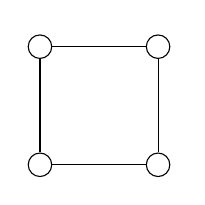
\begin{tikzpicture}[node distance=2cm, on grid, auto,
    state/.style={draw, circle, inner sep=3pt}]
        \node[state] (q0) {};
        \node[state, right=1.5of q0] (q1) {};
        \node[state, below=1.5of q0] (q2) {};
        \node[state, right=1.5of q2] (q3) {};
        
        \path
        (q0) edge node {} (q1)
        (q0) edge node {} (q2)
        (q1) edge node {} (q3)
        (q2) edge node {} (q3);
    \end{tikzpicture}
    \end{center}
    
    si indichi se possibile modellare la colorazione $\{0,1\}$ per ciascun nodo, in modo che \textit{vertici adiacenti non abbiano lo stesso colore}. 

    %% INDEX
    \addcontentsline{toc}{subsection}{Esercizio 5.} 
    %%
    \item \textbf{\textcolor{blue}{Esercizio 5.} (**)}\\ 
    Si consideri il del precedente esercizio: si scriva una formula booleana per modellare il problema della colorazione esteso al caso in cui ogni vertice è connesso a ciascun altro vertice, avendo a disposizione un totale di 3 colori.
    
    \begin{center}
    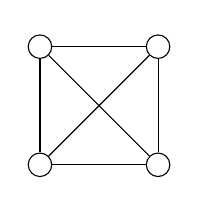
\begin{tikzpicture}[node distance=2cm, on grid, auto,
    state/.style={draw, circle, inner sep=3pt}]
        \node[state] (q0) {};
        \node[state, right=1.5of q0] (q1) {};
        \node[state, below=1.5of q0] (q2) {};
        \node[state, right=1.5of q2] (q3) {};
        
        \path
        (q0) edge node {} (q1)
        (q0) edge node {} (q2)
        (q1) edge node {} (q3)
        (q2) edge node {} (q3)
        (q0) edge node {} (q3)
        (q2) edge node {} (q1);
    \end{tikzpicture}
    \end{center}

    \NewPageHeader

    %% INDEX
    \addcontentsline{toc}{subsection}{Esercizio 6.} 
    %%
    \item \textbf{\textcolor{black}{Esercizio 6.} (***)}\\ 
    Si definisca una formula booleana per modellare un Sudoku 9x9. Si ricorda che:
    \begin{itemize}
        \item Ogni cella può contenere numeri da $1$ a $9$;
        \item Ogni cella deve essere tale che \textit{ogni riga contenga tutti i numeri da 1 a 9}, indipendentemente dall'ordine;
        \item Ogni sottogruppo 3x3 indicato in figura deve contenere tutti i numeri da 1 a 9.
    \end{itemize}


Si ricorda come lo schema del sudoku è il seguente:

\begin{figure}[h]
\begin{center}
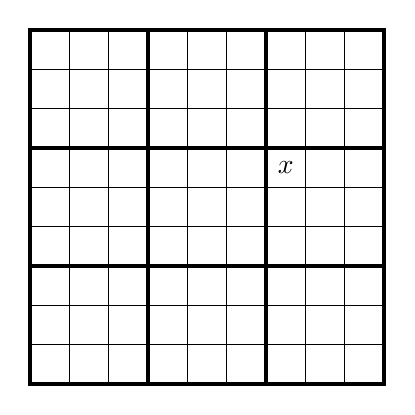
\begin{tikzpicture}[scale=0.5]
  % grid outer
  \draw[line width=1.2pt] (0,0) rectangle (9,9);

  % thin grid lines
  \foreach \i in {1,...,8}{
    \draw[line width=0.4pt] (\i,0) -- (\i,9);
    \draw[line width=0.4pt] (0,\i) -- (9,\i);
  }

  % thick 3x3 separators
  \foreach \k in {0,3,6,9}{
    \draw[line width=1.6pt] (\k,0) -- (\k,9);
    \draw[line width=1.6pt] (0,\k) -- (9,\k);
  }
  \node[] at (6.5,5.5) {$x$};

\end{tikzpicture}
\caption{Sudoku 9×9} 
\end{center}
\end{figure}


Dove si indichi $x = X_{r=4,c=7,k}\ , \quad k\in\{1,2,...,9\}$.
    
\begin{osservazioni}
    \underline{\textit{Soluzione (dettagliata).}}\\
    L'esercizio chiede di costruire una formula booleana tale da modellare il problema del sudoku 9x9. In questo caso, si ricorda che il gioco del sudoku si basa su alcuni vincoli rispetto a \textit{righe, colonne e blocchi 3x3 (selezionati)}. Modellare il problema del sudoku significa allora riuscire a idenfidicare attraverso una formula che catturi tali vincoli e permetta di identificare il valore contenuto in ciascuna delle celle.\\

    Come suggerito dalla consegna, infatti, possiamo indicare con la variabile booleana $$X_{r,c,k}$$ l'informazione $$\text{In\ posizione} (r,c) \text{\ della\ matrice\ è\ contenuto\ il\ numero \ }k$$\\
    
    E, come noto, una \textit{assegnazione delle variabili} (i.e. un modello $\alpha$) per la formula finirebbe per assegnare un \textbf{valore di verità} per ciascuna delle variabili, con $r,c=1,..,9$; ossia $$\alpha(X_{4,5,6})=1,\quad \alpha(X_{6,7,4})=1$$ se e solo se abbiamo

    \begin{center}
    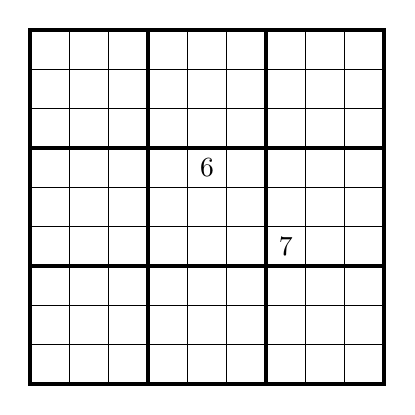
\begin{tikzpicture}[scale=0.5]
      % grid outer
      \draw[line width=1.2pt] (0,0) rectangle (9,9);
    
      % thin grid lines
      \foreach \i in {1,...,8}{
        \draw[line width=0.4pt] (\i,0) -- (\i,9);
        \draw[line width=0.4pt] (0,\i) -- (9,\i);
      }
    
      % thick 3x3 separators
      \foreach \k in {0,3,6,9}{
        \draw[line width=1.6pt] (\k,0) -- (\k,9);
        \draw[line width=1.6pt] (0,\k) -- (9,\k);
      }
    \node[] at (4.5,5.5) {$6$};
    \node[] at (6.5,3.5) {$7$};
    \end{tikzpicture}
    \end{center}

    Non possiamo assumere nulla invece da $$\alpha(X_{4,5,9})=0$$
\end{osservazioni}
\NewPageHeader
\begin{osservazioni}
    se non la conoscenza del fatto che in posizione $(4,5)$ della matrice (i.e. sudoku) non è presente il numero $9$.\\
    
    Prima di considerare i vincoli, per chiarezza, consideriamo quindi che:
    \begin{itemize}
        \item Per ogni posizione del sudoku potremmo inserire un qualsiasi numero da 1 a 9, quindi avremo un totale di $9$ variabili per ciascuna posizione della matrice $(r,c)$.
        \item Poiché $r=1,...,9$ e $c=1,...,9$, allora sono presenti un totale di $9\times 9$ celle, ognuna con $9$ possibili valori di $k$ (cfr. punto 1.).
        \item Quindi, considerando la notazione $X_{r,c,k}$ abbiamo un totale di $9\times9\times9$ variabili.
    \end{itemize}
Ma non avremo bisogno di altro per risolvere il problema richiesto.\\

\underline{\textbf{Presentazione dei vincoli}}\\
Dovremo considerare, per rendere propria la matrice del Sudoku i seguenti vincoli definiti sui valori delle celle -dunque sulle variabili booleane presentate precedentemente-:
\begin{enumerate}
    \item Ogni cella deve contenere necessariamente \textbf{uno} (1) e \textbf{un solo} (2)valore.
    \item Ogni \textbf{riga} deve contenere necessariamente \textbf{tutti i numeri da 1 a 9} (indipendentemente dall'ordine)
    \item Ogni \textbf{colonna} deve contenere necessariamente \textbf{tutti i numeri da 1 a 9} (indipendentemente dall'ordine)
    \item Ogni \textbf{blocco} evidenziato 3x3 deve contenere necessariamente \textbf{tutti i numeri da 1 a 9} (indipendentemente dall'ordine)
\end{enumerate}
Possiamo considerare ognuno dei vincoli indipendentemente: alla fine, poiché sono \textit{caratteristiche} che devono essere verificate tutte insieme per rendere proprio il problema, sarà sufficiente legare con $\land$ le rispettive formule booleane.\\
Consideriamo nell'ordine presentato i vincoli, per semplicità.\\

\underline{\textbf{1. Vincolo sulle righe}}\\
Il sudoku impone che, in ogni riga, sia presente, indipendentemente dall'ordine, ogni numero da 1 a 9. Quindi, molte configurazioni possono essere trovate, come:

  \begin{center}
    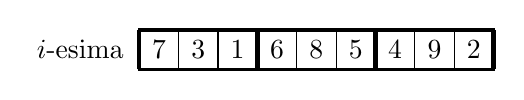
\begin{tikzpicture}[scale=0.5]
      % grid outer
      \draw[line width=1.2pt] (0,0) rectangle (9,1);
    
      % thin grid lines
      \foreach \i in {1,...,8}{
        \draw[line width=0.4pt] (\i,0) -- (\i,1);
        %\draw[line width=0.4pt] (0,\i) -- (9,\i);
      }
    
      % thick 3x3 separators
      \foreach \k in {0,3,6,9}{
        \draw[line width=1.6pt] (\k,0) -- (\k,1);
      %  \draw[line width=1.6pt] (0,\k) -- (9,\k);
      }
    \node[] at (1.5,0.5) {$3$};
    \node[] at (2.5,0.5) {$1$};
    \node[] at (3.5,0.5) {$6$};
    \node[] at (4.5,0.5) {$8$};
    \node[] at (5.5,0.5) {$5$};
    \node[] at (6.5,0.5) {$4$};
    \node[] at (7.5,0.5) {$9$};
    \node[] at (8.5,0.5) {$2$};
    \node[] at (0.5,0.5) {$7$};
    \node[] at (-1.5,0.5) {$i$-esima};
    \end{tikzpicture}
    \end{center}

    Fissiamo quindi, come nell'esempio, la riga ad essere la $i$-esima. Tutte le posizioni della riga sono ottenute variando la colonna -il secondo indice-. Allora l'esempio precedente, secondo la nostra notazione, può essere tradotto come il fatto che il modello associ un valore di verità a ciascuna delle variabili che rappresentano la situazione indicata, ossia, rispettivamente:
    $$X_{i,1,7}\quad X_{i,2,3}\quad X_{i,3,1}\quad X_{i,4,6}\quad X_{i,5,8}\quad X_{i,6,5} \quad ... \quad X_{i,9,2}$$

    Ragioniamo allora sul vincolo, così da poterlo ri-esprimere in termini delle variabili:
    di fatto, stiamo chiedendo che in ogni cella $$(i,c),\quad c=1,...,9$$ di questa riga sia presente un numero \textit{diverso rispetto a tutti i numeri delle altre celle} della stessa riga. Se però è vero che ogni cella ha un solo numero, unico rispetto alla riga, sarà vero anche che ogni numero è presente \textbf{una sola volta all'interno della riga}: fissando un $k=1,..,9$, esso potrà essere presente una sola volta all'interno della riga.\\

    Perché questo è importante? Perché avendo fissato la riga $i$ e il numero di interesse da inserire $k$, l'unico indice libero è proprio $c$, che identifica \textbf{quale cella stiamo considerando}. Allora, ricordando che per definiizione tutte le variabili 
    $$X_{\mathbf{i},c,\mathbf{k}},\quad c=1,...,9$$
    stanno \textbf{affermando} che:
    $$\text{In\ posizione} (r,c) \text{\ della\ matrice\ è\ contenuto\ il\ numero \ }k$$
    Risulterà immediato pensare che \textbf{solo ad una tra queste variabili potrà essere assegnato a un valore di verità 1, affinché il vincolo sia verificato}, perché \textit{solo in una delle posizioni della riga -i.e. $(i,c)$, $c$ variabile- può essere effettivamente contenuto il valore $k$!}\\

    Con questo chiaro, sappiamo che \textbf{imporre il vincolo} sulle righe significa semplicemente riuscire ad imporre che il modello dica che \textbf{solo una} di queste variabili:
    $$X_{\mathbf{i},c,\mathbf{k}}$$
    "\textit{vera}", mentre le altre come "\textit{false}", proprio grazie al fatto che ognuna di queste variabili sta affermando qualcosa; solo in un caso può essere vero che è contenuto il simbolo $k$ nella cella correntemente considerata. \\

    Ma allora, se solo in una cella è vero che è contenuto il numero $k$, assumendo che \textbf{ognuna abbia un numero} -lo scriveremo dopo-, significa che, prese due celle,  \textbf{non possiamo accettare che sia l'una che l'altra lo contengano allo stesso tempo} o che \textbf{o è l'una a non contenere il numero k o è l'altra a non contenerlo.} 

    $$Idea: \quad \overline{\bigg(X_{i,c_2,k}\land X_{r,c_2,k}\bigg)} \quad \equiv \quad \overline X_{i,c_1,k} \lor \overline X_{i,c_2,k} $$

\end{osservazioni}
\NewPageHeader
\begin{osservazioni} 

    Però, questo \textbf{deve valere allo stesso tempo} per \textbf{ogni} coppia $c_1,c_2$; l'operatore and si occupa proprio di imporre la verità di tutte le condizioni:
         



    $$\begin{array}{c}
         \bigg(\overline X_{i,1,k} \lor \overline X_{i,2,k}\bigg) \land \\
         \bigg(\overline X_{i,1,k} \lor \overline X_{i,3,k}\bigg) \land \\
         ... \\
         \bigg(\overline X_{i,2,k} \lor \overline X_{i,3,k}\bigg) \land \\
         ...  \\ 
         \\
    \end{array}$$
    
    $$\begin{array}{c}
    = \bigwedge\limits_{\begin{array}{c}
         c_1\ne c_2  \\
         c_1,c_2 \in \{1,...,9\}
    \end{array}} (\overline X_{i,c_1,k} \lor \overline X_{i,c_2,k})
    \end{array}$$

    Non vogliamo però questo sia vero anche per tutte le righe $i=1,...,9$? Questa condizione su una riga generica $i$ deve valere per tutte le scelte di righe,\textbf{ allo stesso tempo}:

             $$\bigwedge\limits_{i=1}^{9}\ \bigg( 
    \bigwedge\limits_{c_1\ne c_2} (\overline X_{i,c_1,k} \lor \overline X_{i,c_2,k})
    \bigg)$$


    Non vorremmo anche che questa condizione che vale per tutte le righe e per un numero $k$ fissato valesse per tutte le scelte di $k$, \textbf{allo stesso tempo}?

    $$\bigwedge\limits_{k=1}^{9}\ \bigg(\bigwedge\limits_{i=1}^{9}\ \bigg( \bigwedge\limits_{c_1\ne c_2} (\overline X_{i,c_1,k} \lor \overline X_{i,c_2,k})
    \bigg)\bigg)$$

    Ecco allora che il vincolo è stato riscritto. Possiamo convincerci del fatto che:
    \begin{itemize}
        \item Se solo una tra le celle $(i,c_1)$ e $(i,c_2)$ contiene il numero $k$, allora solo una tra $X_{i,c_1,k}$ e $X_{i,c_2,k}$ sarà vera. Se così, solo una tra $\overline X_{i,c_1,k}$ e $\overline X_{i,c_2,k}$ sarà falsa e l'\textit{or} verificato (True).
        \item Se nessuna delle due celle lo contiene, entrambe $\overline X_{i,c_1,k}$ e $\overline X_{i,c_2,k}$ saranno vere e l'\textit{or} verificato.
        \item Nel vero caso problematico, ossia se più celle distinte contengono il numero $k$... significherà che, ad esempio, sia $X_{i,c_1,k}$ che $X_{i,c_2,k}$ saranno affermazioni con assegnazione a True, ma allora sia $\overline X_{i,c_1,k}$ che $\overline X_{i,c_2,k}$ saranno affermazioni false. Allora, la clausola finirebbe per essere falsa: questo non può accaadere perché il modello deve necessariamente verificare questa clausola che è legata con \textbf{and} a tutte le altre! Quindi, non accadrà mai per un modello che soddisferà la formula booleana.
    \end{itemize}

    Non è forse quanto chiede il vincolo? Sì, perché due celle non possono contenere lo stesso numero, ma due celle diverse della riga possono entrambe possono entrambe non contenerlo. L'unico caso che non soddisfa la formula sarebbe quando due celle contengono entrambe lo stesso numero.
    Sarà proprio il chiedere che 
    \begin{itemize}
        \item \textbf{ogni cella abbia un numero}
        \item \textbf{su due celle non possa esserci lo stesso numero}
    \end{itemize}
    A forzare l'imposizione del vincolo.

    Fino ad ora abbiamo quindi:

    $$\phi_{righe}= \bigwedge\limits_{k=1}^{9}\ \bigg(\bigwedge\limits_{r=1}^{9}\ \bigg( 
    \bigwedge\limits_{c_1\ne c_2} (\overline X_{r,c_1,k} \lor \overline X_{r,c_2,k})
    \bigg)\bigg)$$\\
    

\underline{\textbf{2. Vincolo di presenza e unicità di un numero}}\\
Prima abbiamo assunto vero questa proprietà, ma ora possiamo effettivamente imporla. Possiamo imporre che in ciascuna cella sia presente almeno un numero: per ogni cella, fissando $r$ e $c$, almeno un numero tra i nove disponibili deve essere presente. Allora, almeno una delle affermazioni della forma \textit{"nella cella $(r,c)$ è presente il numero $k$} dovrà essere vera:

    $$\phi_{presenza}= \bigwedge\limits_{r=1}^{9}\ \bigwedge\limits_{c=1}^{9}\ \bigg( 
    \bigvee\limits_{k=1}^9 X_{r,c,k}
    \bigg)$$\\

Questo però non vieta la possibilità che siano \textit{tutte indicate come "affermazioni" vere} da una assegnazione per la formula. Questo impone che almeno un numero sia presente, ma non vieta la sovrapposizione...\\

La formula sopra quindi può essere soddisfatta anche da una assegnazione delle variabili in cui 
$$\alpha(X_{r,c,1})=1,\quad \alpha(X_{r,c,2})=1,\quad...\quad \alpha(X_{r,c,1})=1\quad$$

\end{osservazioni}
\NewPageHeader
\begin{osservazioni}

Non abbiamo infatti imposto l'\textit{unicità} delle quantità contenute nella cella: questo può essere espresso a parole dicendo che, analogamente:

\begin{itemize}
    \item \textit{Non possiamo accettare che contemporaneamente ci sia $X_{r,c,k_1}$ e $X_{r,c,k_2}$}: $\overline{\bigg(X_{r,c,k_1}\land X_{r,c,k_2}\bigg)}$
    \item \textit{Se non ci sono entrambi i numeri, allora o non è presente uno o non è presente l'altro $\bigg( \overline X_{r,c,k_1}$ e $\overline X_{r,c,k_2} \bigg)$}
\end{itemize}

Allora, questa informazione dovrà valere per ogni scelta di $r,c$ e per ogni valore $k_1\ne k_2$:

    $$\phi_{unicità}= \bigwedge\limits_{r=1}^{9}\ \bigwedge\limits_{c=1}^{9}\ \bigg( 
    \bigwedge\limits_{k_1\ne k_2} ( \overline X_{r,c,k_1} \lor\overline X_{r,c,k_2} )
    \bigg)$$\\

Così, quindi, abbiamo imposto che ogni cella può avere uno ed un solo numero.

\underline{\textbf{3. Vincolo sulle colonne}}\\
Grazie al precedente lavoro e alla simmetria, il vincolo sulle colonne è immediato, a meno di scambiare righe e colonne:

$$\phi_{colonne}= \bigwedge\limits_{k=1}^{9}\ \bigg(\bigwedge\limits_{c=1}^{9}\ \bigg( 
    \bigwedge\limits_{r_1\ne r_2} (\overline X_{r_1,c,k} \lor \overline X_{r_2,c,k})
    \bigg)\bigg)$$\\

\underline{\textbf{4. Vincolo sui blocchi}}\\
Per un sudoku vengono introdotti anche vincoli su blocchi 3x3, chiedendo che siano presenti tutti i numeri da $1$ a $9$ al suo interno:

    \begin{center}
    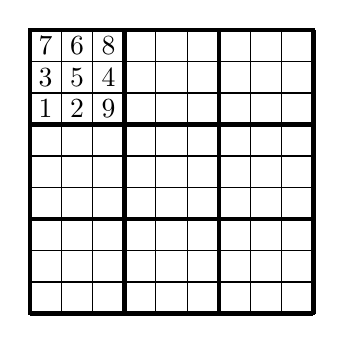
\begin{tikzpicture}[scale=0.4]
      % grid outer
      \draw[line width=1.2pt] (0,0) rectangle (9,9);
    
      % thin grid lines
      \foreach \i in {1,...,8}{
        \draw[line width=0.4pt] (\i,0) -- (\i,9);
        \draw[line width=0.4pt] (0,\i) -- (9,\i);
      }
    
      % thick 3x3 separators
      \foreach \k in {0,3,6,9}{
        \draw[line width=1.6pt] (\k,0) -- (\k,9);
        \draw[line width=1.6pt] (0,\k) -- (9,\k);
      }
    \node[] at (0.5,8.5) {$7$};
    \node[] at (0.5,7.5) {$3$};
    \node[] at (0.5,6.5) {$1$};
    
    \node[] at (1.5,8.5) {$6$};
    \node[] at (1.5,7.5) {$5$};
    \node[] at (1.5,6.5) {$2$};

    \node[] at (2.5,8.5) {$8$};
    \node[] at (2.5,7.5) {$4$};
    \node[] at (2.5,6.5) {$9$};
    \end{tikzpicture}
    \end{center}


A questo punto, possiamo definire formalmente i blocchi, quali sottoinsiemi di celle, ognuna identificata dalla corrispondente riga e colonna:

$$B_{i,j} = \{\  (r,c) \mid r\in \{3i+1,3i+2,3i+3\}, \ c\in \{3i+1,3i+2,3i+3\} \ \}, \quad \ i,j\in\{0,1,2\}$$

Dove allora il blocco in figura è il primo in alto a sinistra, identificato da $$B_{0,0}=\bigg\{  {\begin{array}{c}
     (1,1),\ (1,2),\ (1,3)  \\
     (2,1),\ (2,2),\ (2,3)  \\
     (3,1),\ (3,2),\ (3,3)\\
\end{array}} \bigg\} $$

A questo punto riconosciamo che il vincolo è il medesimo di quanto espresso per righe e colonne, ma cambiano solo i range di righe e colonne stessi; ora gli indici sarà sufficiente rientrino in quanto evidenziato dal \textbf{blocco corrente}. L'idea è che non più siano controllate solo le celle di una riga o di una colonna, ma del blocco: i parametri $r$ e $c$ cambieranno insieme.\\

A differenza del caso precedente, però, non possiamo chiedere che $r_1\ne r_2 \ e \ c_1\ne c_2$, in quanto le uniche scelte sarebbero i termini sulla diagonale. Considereremo invece \textbf{coppie $(r_1,c_1)$ e $(r_2,c_2)$ appartenenti al blocco $B_{i,j}$}:

    $$... \bigwedge\limits_{\begin{array}{c}
         (r_1,c_1)\ne(r_2,c_2)\\
         (r_1,c_1),(r_2,c_2)\in B_{i,j}
    \end{array}} (\overline X_{r_1,c_1,k} \lor \overline X_{r_2,c_2,k})
    $$\\

Ma questo ci impone di considerare \textbf{tutti} i blocchi -analogamente a prima, per \textit{tutte} le righe o colonne-:

$$... \bigwedge\limits_{i=0}^2\ \bigwedge\limits_{j=0}^2\bigg(\bigwedge\limits_{\begin{array}{c}
         (r_1,c_1)\ne(r_2,c_2)\\
         (r_1,c_1),(r_2,c_2)\in B_{i,j}
    \end{array}} (\overline X_{r_1,c_1,k} \lor \overline X_{r_2,c_2,k})
    \bigg)\bigg)$$\\

\end{osservazioni}
\NewPageHeader
\begin{osservazioni}

E, analogamente, per tutte le scelte di numeri:

$$\bigwedge\limits_{k=1}^9\bigg(\ \bigwedge\limits_{i=0}^2\ \bigwedge\limits_{j=0}^2\bigg(\bigwedge\limits_{\begin{array}{c}
         (r_1,c_1)\ne(r_2,c_2)\\
         (r_1,c_1),(r_2,c_2)\in B_{i,j}
    \end{array}} (\overline X_{r_1,c_1,k} \lor \overline X_{r_2,c_2,k})
    \bigg)\bigg)\bigg)$$\\


Quindi, il vincolo è espresso falla seguente formula booleana:

$$\phi_{blocchi}=\bigwedge\limits_{k=1}^9\bigg(\ \bigwedge\limits_{i=0}^2\ \bigwedge\limits_{j=0}^2\bigg(\bigwedge\limits_{\begin{array}{c}
         (r_1,c_1)\ne(r_2,c_2)\\
         (r_1,c_1),(r_2,c_2)\in B_{i,j}
    \end{array}} (\overline X_{r_1,c_1,k} \lor \overline X_{r_2,c_2,k})
    \bigg)\bigg)\bigg)$$\\


\underline{\textbf{Formula Booleana}}\\
La formula booleana finale può essere ottenuta come 
$$\phi=\phi_{righe}\land \phi_{colonne}\land \phi_{blocchi}\land \phi_{presenza} \land \phi_{unicità}=$$
$$\bigwedge\limits_{k=1}^{9}\ \bigg(\bigwedge\limits_{r=1}^{9}\ \bigg( 
    \bigwedge\limits_{c_1\ne c_2} (\overline X_{r,c_1,k} \lor \overline X_{r,c_2,k})
    \bigg)\bigg) \land 
    \bigwedge\limits_{k=1}^{9}\ \bigg(\bigwedge\limits_{c=1}^{9}\ \bigg( 
    \bigwedge\limits_{r_1\ne r_2} (\overline X_{r_1,c,k} \lor \overline X_{r_2,c,k})
    \bigg)\bigg)$$
    $$\land$$
    $$\bigwedge\limits_{k=1}^9\bigg(\ \bigwedge\limits_{i=0}^2\ \bigwedge\limits_{j=0}^2\bigg(\bigwedge\limits_{\begin{array}{c}
         (r_1,c_1)\ne(r_2,c_2)\\
         (r_1,c_1),(r_2,c_2)\in B_{i,j}
    \end{array}} (\overline X_{r_1,c_1,k} \lor \overline X_{r_2,c_2,k})
    \bigg)\bigg)\bigg)\land $$
    $$\land$$
    $$\bigwedge\limits_{r=1}^{9}\ \bigwedge\limits_{c=1}^{9}\ \bigg( 
    \bigvee\limits_{k=1}^9 X_{r,c,k}
    \bigg)\land \bigwedge\limits_{r=1}^{9}\ \bigwedge\limits_{c=1}^{9}\ \bigg( 
    \bigwedge\limits_{k_1\ne k_2} ( \overline X_{r,c,k_1} \lor\overline X_{r,c,k_2} )
    \bigg)$$\\
\end{osservazioni}



\NewPageHeader

\begin{osservazioni2} 

\underline{\textbf{\textcolor{blue}{Esempio ed intuizione.}}}\\

L'esercizio si conclude, proponendo una formula booleana per la rappresentazione dei vincoli per definire uno schema di sudoku -quale matrice $9\times 9$-. Facendo un salto nella teoria del corso, si può mostrare \textbf{dove può risiedere l'utilità pratica di questo tipo di operazioni}, considerando un gioco o problema a tutti noto. \\

A partire da formule booleane, si ci si può ricondure a uno speciale formato, chiamato \href{https://jix.github.io/varisat/manual/0.2.0/formats/dimacs.html}{\textit{\textcolor{blue}{\underline{DIMACS}}}}, in cui una formula booleana può essere riportata. Si tratta solamente di un formato standard per fornire ad un \textbf{satsolver} una formula CNF ad un sat solver.\\

Un esempio può essere il seguente:
\begin{osservazioni}
\begin{verbatim}
    c questo è un commento
    c inizio della descrizione del problema
    p cnf <num_variabili> <num_clause>

    c ogni clausola rappresenta un letterale, il meno 
    c è la negazione e l'ultimo è 0 per indicare la terminazione:

    c clausola x1 or not x2
    1 -2 0

    c clausola x1 or x2 or not x3
    1 2 -3 0

    c ogni clausola sarà legata con and
\end{verbatim}
\end{osservazioni}

Quindi, come vedremo, potremo
\begin{enumerate}
    \item \textbf{Considerare un problema}, come il sudoku
    \item \textbf{Considerare la sua riformulazione come formula booleana}
    \item \textbf{Fornirla ad un sat-solver}
\end{enumerate}
Tutto per poter alla fine ottenere non solo una assegnazione che verifichi il problema, bensì anche una \textbf{assegnazione per le variabili} che verifichi il problema.\\
%\hline
$$\\$$
Consideriamo un'istanza del problema del sudoku, quale una matrice da ricostruire:

\begin{center}
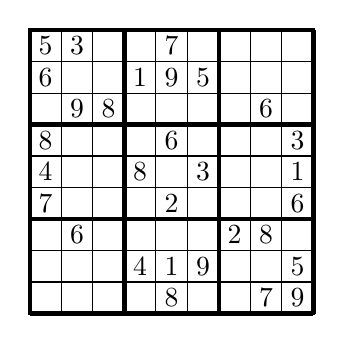
\begin{tikzpicture}[scale=0.4]
  % grid outer
  \draw[line width=1.2pt] (0,0) rectangle (9,9);

  % thin grid lines
  \foreach \i in {1,...,8}{
    \draw[line width=0.4pt] (\i,0) -- (\i,9);
    \draw[line width=0.4pt] (0,\i) -- (9,\i);
  }

  % thick 3x3 separators
  \foreach \k in {0,3,6,9}{
    \draw[line width=1.6pt] (\k,0) -- (\k,9);
    \draw[line width=1.6pt] (0,\k) -- (9,\k);
  }

  %---- ESEMPIO DI SUDOKU ----
  % riga 1
  \node[] at (0.5,8.5) {5};
  \node[] at (1.5,8.5) {3};
  \node[] at (4.5,8.5) {7};

  % riga 2
  \node[] at (0.5,7.5) {6};
  \node[] at (3.5,7.5) {1};
  \node[] at (4.5,7.5) {9};
  \node[] at (5.5,7.5) {5};

  % riga 3
  \node[] at (1.5,6.5) {9};
  \node[] at (2.5,6.5) {8};
  \node[] at (7.5,6.5) {6};

  % riga 4
  \node[] at (0.5,5.5) {8};
  \node[] at (4.5,5.5) {6};
  \node[] at (8.5,5.5) {3};

  % riga 5
  \node[] at (0.5,4.5) {4};
  \node[] at (3.5,4.5) {8};
  \node[] at (5.5,4.5) {3};
  \node[] at (8.5,4.5) {1};

  % riga 6
  \node[] at (0.5,3.5) {7};
  \node[] at (4.5,3.5) {2};
  \node[] at (8.5,3.5) {6};

  % riga 7
  \node[] at (1.5,2.5) {6};
  \node[] at (6.5,2.5) {2};
  \node[] at (7.5,2.5) {8};

  % riga 8
  \node[] at (3.5,1.5) {4};
  \node[] at (4.5,1.5) {1};
  \node[] at (5.5,1.5) {9};
  \node[] at (8.5,1.5) {5};

  % riga 9
  \node[] at (4.5,0.5) {8};
  \node[] at (7.5,0.5) {7};
  \node[] at (8.5,0.5) {9};
\end{tikzpicture}
\end{center}

Dal momento che sappiamo il valore di alcune celle e conosciamo la formula booleana che impone i vincoli della matrice, possiamo imporre e \textbf{aggiungere come vincoli il valore di verità delle variabili corrispondenti alle celle note} (legandole con and alla formula):
$$\phi_{valori\ presenti} = X_{1,1,5} \land X_{1,2,3} \land ... \land X_{9,9,9}$$
\\
Questo, dato che compariranno da sole, imporrà ad \textbf{ogni assegnazione } $\alpha$ delle variabili che tutti i letterali di $phi_{valori\ presenti}$ abbiano come valore di verità $1$. Utilizzando un \textit{sat-solver}, dunque, su:
$$\phi'=\phi_{sudoku}\land \phi_{valori\ presenti}$$
tale che:
$$\alpha \models \phi'$$
possiamo ottenere una \textbf{assegnazione delle variabili che tenga conto sia} dei \textbf{vincoli intrinsechi al gioco, sia} \textbf{delle quantità già presenti nella "tabella"}...

\end{osservazioni2}
\NewPageHeader
\begin{osservazioni2}
... fornendoci dunque una assegnazione delle variabili che altro non è se non la \textbf{soluzione al sudoku fornito}! 

$$$$

\begin{center}
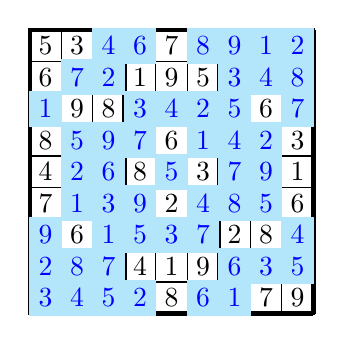
\begin{tikzpicture}[scale=0.4]
  % grid outer
  \draw[line width=1.2pt] (0,0) rectangle (9,9);

  % thin grid lines
  \foreach \i in {1,...,8}{
    \draw[line width=0.4pt] (\i,0) -- (\i,9);
    \draw[line width=0.4pt] (0,\i) -- (9,\i);
  }

  % thick 3x3 separators
  \foreach \k in {0,3,6,9}{
    \draw[line width=1.6pt] (\k,0) -- (\k,9);
    \draw[line width=1.6pt] (0,\k) -- (9,\k);
  }

  %---- ESEMPIO DI SUDOKU ----
  % riga 1
  \node[] at (0.5,8.5) {5};
  \node[] at (1.5,8.5) {3};
  \node[] at (4.5,8.5) {7};

  % riga 2
  \node[] at (0.5,7.5) {6};
  \node[] at (3.5,7.5) {1};
  \node[] at (4.5,7.5) {9};
  \node[] at (5.5,7.5) {5};

  % riga 3
  \node[] at (1.5,6.5) {9};
  \node[] at (2.5,6.5) {8};
  \node[] at (7.5,6.5) {6};

  % riga 4
  \node[] at (0.5,5.5) {8};
  \node[] at (4.5,5.5) {6};
  \node[] at (8.5,5.5) {3};

  % riga 5
  \node[] at (0.5,4.5) {4};
  \node[] at (3.5,4.5) {8};
  \node[] at (5.5,4.5) {3};
  \node[] at (8.5,4.5) {1};

  % riga 6
  \node[] at (0.5,3.5) {7};
  \node[] at (4.5,3.5) {2};
  \node[] at (8.5,3.5) {6};

  % riga 7
  \node[] at (1.5,2.5) {6};
  \node[] at (6.5,2.5) {2};
  \node[] at (7.5,2.5) {8};

  % riga 8
  \node[] at (3.5,1.5) {4};
  \node[] at (4.5,1.5) {1};
  \node[] at (5.5,1.5) {9};
  \node[] at (8.5,1.5) {5};

  % riga 9
  \node[] at (4.5,0.5) {8};
  \node[] at (7.5,0.5) {7};
  \node[] at (8.5,0.5) {9};

\node[, color=blue, fill=cyan!30, fill=cyan!30] at (2.5,8.5) {4};
\node[, color=blue, fill=cyan!30] at (3.5,8.5) {6};
\node[, color=blue, fill=cyan!30] at (5.5,8.5) {8};
\node[, color=blue, fill=cyan!30] at (6.5,8.5) {9};
\node[, color=blue, fill=cyan!30] at (7.5,8.5) {1};
\node[, color=blue, fill=cyan!30] at (8.5,8.5) {2};

\node[, color=blue, fill=cyan!30] at (1.5,7.5) {7};
\node[, color=blue, fill=cyan!30] at (2.5,7.5) {2};
\node[, color=blue, fill=cyan!30] at (6.5,7.5) {3};
\node[, color=blue, fill=cyan!30] at (7.5,7.5) {4};
\node[, color=blue, fill=cyan!30] at (8.5,7.5) {8};

\node[, color=blue, fill=cyan!30] at (0.5,6.5) {1};
\node[, color=blue, fill=cyan!30] at (3.5,6.5) {3};
\node[, color=blue, fill=cyan!30] at (4.5,6.5) {4};
\node[, color=blue, fill=cyan!30] at (5.5,6.5) {2};
\node[, color=blue, fill=cyan!30] at (6.5,6.5) {5};
\node[, color=blue, fill=cyan!30] at (8.5,6.5) {7};

\node[, color=blue, fill=cyan!30] at (1.5,5.5) {5};
\node[, color=blue, fill=cyan!30] at (2.5,5.5) {9};
\node[, color=blue, fill=cyan!30] at (3.5,5.5) {7};
\node[, color=blue, fill=cyan!30] at (5.5,5.5) {1};
\node[, color=blue, fill=cyan!30] at (6.5,5.5) {4};
\node[, color=blue, fill=cyan!30] at (7.5,5.5) {2};

\node[, color=blue, fill=cyan!30] at (1.5,4.5) {2};
\node[, color=blue, fill=cyan!30] at (2.5,4.5) {6};
\node[, color=blue, fill=cyan!30] at (4.5,4.5) {5};
\node[, color=blue, fill=cyan!30] at (6.5,4.5) {7};
\node[, color=blue, fill=cyan!30] at (7.5,4.5) {9};

\node[, color=blue, fill=cyan!30] at (1.5,3.5) {1};
\node[, color=blue, fill=cyan!30] at (2.5,3.5) {3};
\node[, color=blue, fill=cyan!30] at (3.5,3.5) {9};
\node[, color=blue, fill=cyan!30] at (5.5,3.5) {4};
\node[, color=blue, fill=cyan!30] at (6.5,3.5) {8};
\node[, color=blue, fill=cyan!30] at (7.5,3.5) {5};

\node[, color=blue, fill=cyan!30] at (0.5,2.5) {9};
\node[, color=blue, fill=cyan!30] at (2.5,2.5) {1};
\node[, color=blue, fill=cyan!30] at (3.5,2.5) {5};
\node[, color=blue, fill=cyan!30] at (4.5,2.5) {3};
\node[, color=blue, fill=cyan!30] at (5.5,2.5) {7};
\node[, color=blue, fill=cyan!30] at (8.5,2.5) {4};

\node[, color=blue, fill=cyan!30] at (0.5,1.5) {2};
\node[, color=blue, fill=cyan!30] at (1.5,1.5) {8};
\node[, color=blue, fill=cyan!30] at (2.5,1.5) {7};
\node[, color=blue, fill=cyan!30] at (6.5,1.5) {6};
\node[, color=blue, fill=cyan!30] at (7.5,1.5) {3};
\node[, color=blue, fill=cyan!30] at (8.5,1.5) {5};

\node[, color=blue, fill=cyan!30] at (0.5,0.5) {3};
\node[, color=blue, fill=cyan!30] at (1.5,0.5) {4};
\node[, color=blue, fill=cyan!30] at (2.5,0.5) {5};
\node[, color=blue, fill=cyan!30] at (3.5,0.5) {2};
\node[, color=blue, fill=cyan!30] at (5.5,0.5) {6};
\node[, color=blue, fill=cyan!30] at (6.5,0.5) {1};
 
\end{tikzpicture}
\end{center}
$$$$

\end{osservazioni2}
\end{itemize}

\vfill
\noindent\makebox[\linewidth]{\rule{\linewidth}{0.4pt}}
\end{document}